%% -------------------------------------------------------------------------------------
%% tcc.tex -- MAIN FILE
%% -------------------------------------------------------------------------------------
\documentclass[a4paper,12pt,oneside,brazil]{book}

%% -------------------------------------------------------------------------------------
%% PACKAGES
%% -------------------------------------------------------------------------------------

\usepackage[brazil]{babel}
\usepackage[utf8]{inputenc}
\usepackage[T1]{fontenc}

% Cor
\usepackage[table,dvipsnames]{xcolor}

\usepackage[font={small,it},labelfont=bf]{caption}  % \begin{caption}
\usepackage{subcaption}                             % \begin{subfigure}
\usepackage{csquotes}                               % requerido por {babel}
\usepackage{graphicx}                               % \includegraphics
\usepackage{verbatim}                               % \begin{comment}
\usepackage{fullpage}                               % margens menores
\usepackage{indentfirst}                            % indentação dos 1ºs parágrafos
\usepackage{setspace}                               % \setstretch
\usepackage{afterpage}                              % \afterpage
% \usepackage{layouts}                              % debug dos tamanhos do documento
% \afterpage http://tex.stackexchange.com/q/88657

% \newminted{cpp}
% [chapter] é para numerar usando o capítulo
\usepackage[chapter]{minted}

% Links azuis
\usepackage[unicode,colorlinks=true,linkcolor=blue]{hyperref}

% Desligando a ligatura do 'fi'
% http://www.latex-community.org/forum/viewtopic.php?f=5&t=953#p13896
\usepackage{microtype}
\DisableLigatures{encoding = *, family = *}

% Usa estilo "Natbib" para as referências bibliográficas
\usepackage[backend=biber,bibencoding=utf8,style=numeric-comp]{biblatex}

% \makeglossaries
% http://en.wikibooks.org/wiki/LaTeX/Glossary#Using_defined_terms
% sanitize=none: http://tex.stackexchange.com/a/14930/5125
\usepackage[xindy,toc,sanitize=none]{glossaries}

% http://texblog.org/tag/addcontentsline/
\usepackage[numbib]{tocbibind}

% anotações TODO
\usepackage[colorinlistoftodos,portuguese]{todonotes}

% padding de imagens
%\setlength\fboxsep{2mm}

%%%%%%%%%%%%%%%%%%%%%%%%%%%%%%%%%%%%%%%%%%%%%%%%%%%%%%%%%%%%%%%
% Links só nos primeiros usos de gls etc
% http://tex.stackexchange.com/a/109137/5125
%%%%%%%%%%%%%%%%%%%%%%%%%%%%%%%%%%%%%%%%%%%%%%%%%%%%%%%%%%%%%%%
% \usepackage{etoolbox}
% \makeatletter
%% patch first occurence of
%% "\@gls@link[#1]{#2}{\@glo@text}", as
%% this is the one for \glsused{#2}
%\patchcmd{\@gls@}
%  {\@gls@link[#1]{#2}{\@glo@text}}
%  {\@gls@link[#1,hyper=false]{#2}{\@glo@text}}
%  {}{}
%
%\patchcmd{\@Gls@}
%  {\@gls@link[#1]{#2}}
%  {\@gls@link[#1,hyper=false]{#2}}
%  {}{}
%
%\patchcmd{\@GLS@}
%  {\@gls@link[#1]{#2}{\MakeUppercase{\@glo@text}}}
%  {\@gls@link[#1,hyper=false]{#2}{\MakeUppercase{\@glo@text}}}
%  {}{}
%\makeatother
%%%%%%%%%%%%%%%%%%%%%%%%%%%%%%%%%%%%%%%%%%%%%%%%%%%%%%%%%%%%%%%

%% -------------------------------------------------------------------------------------
%% CONFIGURATIONS
%% -------------------------------------------------------------------------------------

%%%%%%%%%%%%%%%%%%%%%
%  ???
%%%%%%%%%%%%%%%%%%%%%
% from http://tex.stackexchange.com/q/57151
%\usepackage{accsupp}
%\newcommand{\emptyaccsupp}[1]{\BeginAccSupp{ActualText={}}#1\EndAccSupp{}}

\addbibresource{bibliografia.bib}

\loadglsentries{glossario.tex}
\makeglossaries

% Seta pasta de figuras
\graphicspath{{Figures/}{Figures/chap3/}}

\includeonly{
    Chapters/Chapter1,     % 1. Introdução
    Chapters/Chapter2,     % 2. Histórico
    Chapters/Chapter3,     % 3. Anatomia
    Chapters/Chapter4,     % 4. Parte técnica
    Chapters/Chapter5,     % 5. Conclusão
    Chapters/Chapter6,     % 6. Referências
    Chapters/Chapter7,     % 7. Parte Subjetiva
}

\hypersetup{
     colorlinks   = true,
     citecolor    = Sepia
}

% Fonte 'Times' do sistema (mais bonita)
% http://www.tug.org/pracjourn/2006-1/schmidt/schmidt.pdf
\renewcommand{\rmdefault}{ptm}

%%%%%%%%%%%%%%%%%%%%%%%%%%%%%%%%%
% Do manual do todonote
%%%%%%%%%%%%%%%%%%%%%%%%%%%%%%%%%
\newcommand{\todorefs}[1]{
    \todo[
        color=Orchid,
        bordercolor=Plum,
        inline
    ]{#1}
}

\newcommand{\todoquestion}[1]{
    \todo[
        color=LimeGreen,
        bordercolor=OliveGreen,
        inline
    ]{#1}
}

\newcommand{\todoerrors}[1]{
    \todo[
        color=BrickRed,
        bordercolor=BrickRed,
        inline
    ]{#1}
}

\newcommand{\todoimg}[1]{
    \missingfigure{#1}
}
%%%%%%%%%%%%%%%%%%%%%%%%%%%%%%%%%

%%%%%%%%%%%%%%%%%%%%%
%  Minted
%%%%%%%%%%%%%%%%%%%%%

% Do manual do minted
\renewcommand\listingscaption{Código-fonte}
\renewcommand\listoflistingscaption{Lista de Códigos fonte}

% http://tex.stackexchange.com/a/99656/5125
\renewcommand{\listoflistings}{%
    \cleardoublepage
    \phantomsection
    \addcontentsline{toc}{chapter}{\listoflistingscaption}%
    \listof{listing}{\listoflistingscaption}%
}

% usando valores predefinidos
% \begin{cppcode}
% template <typename T>
%   T id(T value) {
%     return value;
%   }
% \end{cppcode}
%
%
% sobrescrevendo valores
% \begin{cppcode*} {linenos=false,frame=single}
% template <typename T>
%   T id(T value) {
%     return value;
%   }
% \end{cppcode*}
%
% labels: http://citeseerx.ist.psu.edu/viewdoc/
%      download?doi=10.1.1.169.9130&rep=rep1&type=pdf

\newmintedfile[cfile]{c}{
    linenos,
    frame=single,
    samepage=true,
    numbersep=6pt,
    baselinestretch=1,
    fontfamily=courier,
    fontsize=\scriptsize
}

%% -------------------------------------------------------------------------------------
%% DOCUMENT
%% -------------------------------------------------------------------------------------

\begin{document}

\thispagestyle{empty}

% Numeração das primeiras páginas em números romanos
\frontmatter

% OBS:
% \clearpage vs \newpage
% http://tex.stackexchange.com/a/45619/5125
%
% \afterpage{\clearpage}
% http://tex.stackexchange.com/q/88657


%%%%%%%%%%%%%%%%%%%%%
%  Capa
%  https://www.sharelatex.com/blog/2013/08/09/thesis-series-pt5.html
%%%%%%%%%%%%%%%%%%%%%
\begin{titlepage}
    \begin{center}
        %\addcontentsline{toc}{chapter}{Capa}
        \vspace*{1cm}

        \Huge
        \textbf{Anatomia do BitTorrent}

        \vspace{0.5cm}
        \LARGE
        a Ciência da Computação por trás do protocolo

        \vspace{2.5cm}

        \textbf{
            Paulo Cheadi Haddad Filho \\
            Orientador: José Coelho de Pina
        }

        \vfill

        Trabalho de Formatura Supervisionado

        \vspace{3.5cm}

        
\includegraphics[scale=0.1]{logo-ime.png}

        \vspace{2cm}

        \Large
        %Instituto de Matemática e Estatística\\
        Universidade de São Paulo\\
        São Paulo, 2013

    \end{center}
    \afterpage{\clearpage}

\end{titlepage}

% Melhor ter fonte menor e espaçamento de linha maior
\setstretch{1.3}



%%%%%%%%%%%%%%%%%%%%%
% Páginas frontais
%%%%%%%%%%%%%%%%%%%%%

% Sumário
\tableofcontents

% Lista de códigos fonte
\listoflistings

% Lista de figuras
\listoffigures

% Glossário
% \glsaddall
\printglossary[type=main,style=altlist]

% Lista de TODOs
\listoftodos
\todototoc

% Lista de abreviações, se precisar
\begin{comment}
    % Tabelas mais fáceis de ler
    \setstretch{1.5}

    % Nova página
    \afterpage{\clearpage}

    % Lista de abreviações (2 colunas)
    \listofsymbols{ll} {
    % \textbf{Acronym} & \textbf{W}hat (it) \textbf{S}tands \textbf{F}or \\
    % \textbf{LAH} & \textbf{L}ist \textbf{A}bbreviations \textbf{H}ere \\
    }

    % Volta pro 1.3
    \setstretch{1.3}
\end{comment}

\afterpage{\clearpage}



%%%%%%%%%%%%%%%%%%%%%
% Conteúdo
%%%%%%%%%%%%%%%%%%%%%

% Tamanhos / Distâncias
% http://tex.stackexchange.com/a/24468/5125
% http://www.las.ic.unicamp.br/pub/ctan/macros/latex/contrib/layouts/layman.pdf
\setlength{\baselineskip}{15pt}                % Entre linhas do texto
\setlength{\parskip}{15pt}                     % Entre parágrafos
\setlength{\textfloatsep}{1.25\baselineskip}   % Entre floats [t] ou [b] e parágrafos
\setlength{\intextsep}{1.25\baselineskip}      % Entre floats [h] e parágrafos
\setlength{\abovecaptionskip}{.3\parskip}      % Acima das legendas
\setlength{\belowcaptionskip}{-\baselineskip}  % Abaixo das legendas
\addtolength{\belowcaptionskip}{1.2ex}
\setlength{\topsep}{0pt}                       % Espaço superior de listas 1
\setlength{\partopsep}{-\baselineskip}         % Espaço superior de listas 2
\addtolength{\partopsep}{1.2ex}

% Numeração normal em indo-arábico
\mainmatter

% Inclusões dos capítulos
%!TEX root = ../tcc.tex

\chapter{Introdução}

Desde o início da história da computação, o compartilhamento de dados é uma ação
naturalmente necessária e que passou a ser mais comum com a criação dos dispositivos de
armazenamento de dados sob a forma de arquivos, com a Internet anos depois e, mais
recentemente, com a computação em nuvem.

À partir de 1999, com o surgimento do Napster, as \glspl{p2p} passaram a ser mais
populares, sendo frequentemente utilizadas para transferir dados. Essas redes têm como
característica principal computadores transferindo dados entre si, ou seja, não
existindo funções fixas de fonte e de consumo de dados, mas sim de ambas essas funções.

O comunicação \gls*{p2p} veio se desenvolvendo ao longo dos anos. Em 2003, esse
desenvolvimento teve um grande impulso, quando Bram Cohen propôs o protocolo BitTorrent,
lançando juntamente com um programa cliente, e incentivando o seu uso por ``testadores''
simplesmente compartilhando material pornográfico. Com isso, pôde melhorar o seu
funcionamento, se tornando popular rapidamente através de seus usuários.

Desde então, muitos programas de compartilhamento BitTorrent passaram a ser
desenvolvidos, e o protocolo foi sendo estudado pela área acadêmica, passando por
melhorias. Em 2013, o protocolo foi o responsável por aproximadamente 10\% do tráfego
total de Internet nos Estados Unidos \cite{report:internet-usage-2013}, se tornando uma
das formas mais eficientes e utilizadas de se compartilhar arquivos via Internet
atualmente.

O BitTorrent contém conceitos de diversos tópicos em Ciência da Computação, tais como
teoria dos jogos, estruturas de dados, tabelas de dispersão, etc, contando ainda com
diversos estudos acadêmicos sobre topologias de rede formadas e otimizações de redes e
algoritmos, por exemplo.

Neste trabalho, estudamos o protocolo BitTorrent, analisando em profundidade a sua
aplicação pelo programa cliente Transmission \cite{site:transmission}, particularmente
interessados nos elementos de Ciência de Computação presentes no código. Este texto
contém uma descrição desses vários elementos encontrados, junto com trechos de código
que consideramos ilustrativos para exemplicá-los.

No final, relacionamos os conceitos de Ciência da Computação encontrados no
Transmission, e onde eles aparecem ou se aparecem na grade curricular do Bacharelado em
Ciência da Computação.

\afterpage{\clearpage} % Introdução

%!TEX root = ../tcc.tex

\chapter{Napster, Gnutella e BitTorrent}

\begin{comment}
Vou contar a história do BitTorrent, desde o aumento do uso de
transferências de dados via internet, passando pela criação de protocolos e softwares
usados para baixar arquivos de forma ilegal, até a sua criação e o boom de usuários que
o utilizam para essa motivação. Em paralelo, discutirei os motivos legais pelos quais os
softwares anteriores foram descontinuados, que influenciaram diretamente na sua criação.

Separarei em 3 períodos: o antes, a criação e as consequências disso no mundo.
\end{comment}

Para entendermos como e por que o BitTorrent se tornou o que é hoje, devemos voltar um
pouco no tempo e rever a história que precedeu à sua criação, que é o fim da década dos
anos 1990.

% http://tex.stackexchange.com/a/99664
% \newglossaryentry{www}{
%     name={World Wide Web},
%     description={World Wide Web (WWW) é nome que se dá à rede mundial de
%             computadores interligados, que originou a Internet},
%     first={World Wide Web (WWW)},
%     long={World Wide Web}
% }

\section{Período pré-torrent}

\newglossaryentry{isp}{
    name={ISP},
    description={do inglês \emph{Internet Service Provider}; fornecedores de
    acesso a Internet, que são empresas que vendem serviço e equipamento que permitem
    o acesso de um computador pessoal acessar a Internet},
    first={fornecedor de acesso a Internet (\glsentryname{isp})},
    long={fornecedor de acesso a Internet},
    plural={\glsentryname{isp}s},
    firstplural={fornecedores de acesso a Internet (\glsentryname{isp})}
}

\newglossaryentry{mp3}{
    name={MP3},
    description={do inglês \emph{MPEG-1/2 Audio Layer 3}; formato patenteado de
    compressão de dados de áudio digital que usa um método de compressão de dados com
    perdas},
    first={\glsentrylong{mp3} (\glsentryname{mp3})},
    long={formato de áudio \glsentryname{mp3}},
    plural={\glsentryname{mp3}s}
}

\cite{site:wiki-fs}
\cite{site:wiki-fs-timeline}

Entre o final dos anos 80 e o início dos 90, a Internet deixou de ser uma rede de
computadores usada somente por entidades governamentais, laboratórios de pesquisa e
universidades, passando a ter seu acesso comercializado para o público em geral pelos
\glspl{isp} \cite{site:wiki-isp}. Com o advento do \gls{mp3} no final de 1991
\todo{Como faz referência a uma coisa deste tipo?} e do seu primeiro reprodutor de
áudio \gls{mp3} \cite{site:wiki-mp3} Winamp, o tráfego da Internet aumentou devido ao aumento da troca direta de arquivos.

Em 1998, dois sites de compartilhamento de músicas foram criados: o AudioGalaxy.com e o
MP3.com, ambos sites de busca de MP3 sobre arquivos que seus usuários
faziam upload. Ambos os sites ajudaram na popularização do MP3 como forma de se escutar
músicas no dia a dia, que foi catalisado quando indústrias de equipamentos eletrônicos
anunciaram seus sucessores do toca- fitas: os tocadores de mídia portáteis, popularmente
conhecidos como MP3 players.

Não demorou muito tempo para a indústria da música, representada pela RIAA (Recording
Industry Association of America, Associação da Indústria de Gravação da América) começar
a enxergar essa popularização do formato MP3 como um perigo real de diminuição de seus
lucros com as vendas de discos, e então passou a encabeçar a frente de combate contra a
troca de arquivos protegidos por direitos autorais pela Internet. Pouco tempo depois,
durante o governo Clinton, o Senado americano aprova uma lei de proteção a conteúdos com
direitos autorais, estabelecendo regras mais específicas sobre esses direitos autorais e
se tornando obstáculo àqueles sites de compartilhamento por penalizar os usuários por
infringir esses direitos.

No segundo semestre de 1999 surgiu o Napster, um serviço de compartilhamento de MP3 que
inovou por desfigurar o modelo cliente-servidor ao possuir conexões entre usuários e não
a servidores, criando assim a primeira rede P2P.

O sucesso foi rápido, e em dezembro de 1999 já enfrentava sua primeira ação judicial,
vinda de várias grandes gravadoras. Sua popularidade foi crescendo, atingindo o auge de
13.6 milhões de usuários em fevereiro de 2001. A sua vida começou a complicar em julho de
2001, quando foi iniciada uma ação judicial por responsabilidade na distribuição de
conteúdo protegido. O caso foi finalizado em setembro de 2001, obrigando a desligar o
serviço de indexação, que tornou a rede P2P indisponível, e ainda a pagar 26 milhões de
dólares por danos já causados e também pelos futuros, fazendo com que pedisse falência.

O sucesso do Napster, mesmo que por curto período tempo, mostrou a eficiência que redes
P2P poderiam ter, e com isso novos softwares e modelos de redes foram sendo lançados,
porém tentando contornar o ponto fraco do antecessor a fim de não serem novos alvos de
medidas judiciais. A solução para isso foi tentar descentralizar o mecanismo de indexação
e busca, que foi o calcanhar de Aquiles do Napster.

A pioneira nessa tentativa foi a rede Gnutella, que foi lançada em 2003 mas que em sua
primeira versão não conseguiu manter o bom desempenho do Napster. A busca era demorada e
inconsistente, pois era repassada aleatória e finitamente de peers para seus izinhos, o
que podia terminar em buscas sem resultados mesmo quando um arquivo estava sendo
compartilhado por alguém conectado à rede.

continua...

\section{Nascimento do BitTorrent}

Aqui contarei a história do surgimento do protocolo.

\section{Mundo pós-torrent}

Aqui discorrerei sobre as consequências do uso do BitTorrent, desde as influências acadêmico-tecnológicas da sua difusão, bem como explicarei as questões jurídicas envolvidas no seu uso.

\clearpage
 % Histórico

%!TEX root = ../tcc.tex

\chapter{Anatomia do BitTorrent}

O BitTorrent é uma rede \gls{p2p}, onde cada um de seus usuários assume o papel híbrido
de servidor (que fornece os arquivos) e de cliente (que adquire os arquivos). Cada
computador é chamado de \gls{peer}.

Cada transferência por BitTorrent está associada a um \gls{torrentfile}, que contém
\glspl{metadata}, que são informações sobre arquivos que constituem um pacote chamado
\gls{torrent}. Além disso, possui um ou mais endereços de \glspl{tracker}, que são
servidores que mantém listas atualizadas dos \glspl*{peer} que estão compartilhando
aqueles arquivos, atualizadas em curtos períodos de tempo (usualmente 30 minutos).

\begin{comment}
    \begin{figure}[ht!]
        \centering
        \fbox{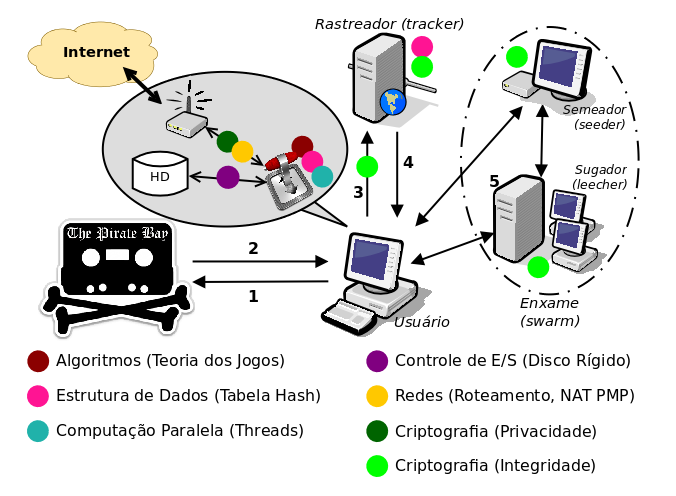
\includegraphics[width=0.64\textwidth]{funcionamento.png}}
        \caption{esquema básico do funcionamento do BitTorrent}
        \label{fig:torrent-basics}
    \end{figure}
\end{comment}

Enquanto um \gls*{peer} estiver fazendo download de um \gls*{torrent}, ele é chamado de
\gls{leecher}, pois ainda consumirá dados de outros \glspl*{peer}; quando o download
acabar, passará a ser um \gls{seeder}, que somente enviará dados.

Os \glspl*{torrentfile} ficam disponíveis em vários sites de índice (às vezes, chamados
de comunidades), como o \href{http://thepiratebay.sx/}{ThePirateBay}, o
\href{http://kickass.to/}{Kickass} ou \href{https://torrentz.eu/}{Torrentz} (muitas
vezes em mais de um deles ao mesmo tempo). Apesar de todo conteúdo compartilhado possuir
um \gls*{torrentfile}, não necessariamente um \gls*{torrentfile} está sendo
compartilhado naquele momento, podendo até mesmo estar extinto.

\Glspl*{peer} que participam do compartilhamento de um \gls*{torrent} específico
fazem parte do \gls{swarm}, onde os dados contidos nesse \gls*{torrent} são
compartilhados por partes com outros \glspl*{peer}.

A quantidade total de partes varia de acordo com cada \gls*{torrent}: o tamanho total
dos arquivos contidos nesse \gls*{torrent} é dividido em blocos de tamanho fixo
(geralmente 256kB) e transmitido de forma independente das outras partes, seguindo uma
ordem estabelecida pelo algoritmo de troca de partes (explicado na seção~\ref{titfortat}).
Essa ordem varia de acordo com o estado atual do \gls*{swarm} desse \gls*{torrent}.

\newpage
\begin{figure}[H]
    \newlength{\myvsize}
    \newlength{\myhsize}
    \setlength{\myvsize}{5mm}
    \setlength{\myhsize}{0.28\textwidth}

    \centering

    \begin{subfigure}[H]{\myhsize}
        \fbox{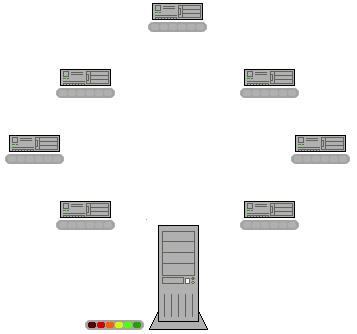
\includegraphics[width=\textwidth]{Torrentcomp_small-0.png}}
        \caption{}
        \label{fig:torrent-repr-0}
    \end{subfigure}%
    \quad %add desired spacing between images (~, \quad, \qquad or blank line)
    \begin{subfigure}[H]{\myhsize}
        \fbox{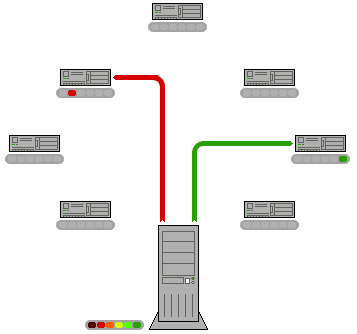
\includegraphics[width=\textwidth]{Torrentcomp_small-1.png}}
        \caption{}
        \label{fig:torrent-repr-1}
    \end{subfigure}%
    \quad
    \begin{subfigure}[H]{\myhsize}
        \fbox{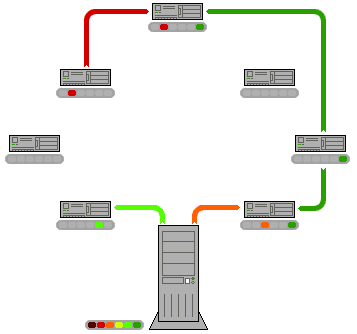
\includegraphics[width=\textwidth]{Torrentcomp_small-2.png}}
        \caption{}
        \label{fig:torrent-repr-2}
    \end{subfigure}

    \vspace{\myvsize}

    \begin{subfigure}[H]{\myhsize}
        \fbox{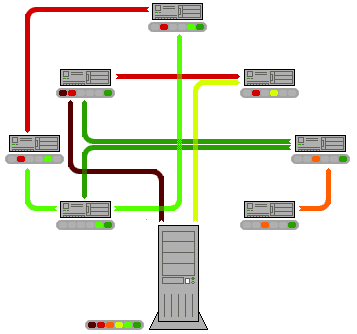
\includegraphics[width=\textwidth]{Torrentcomp_small-3.png}}
        \caption{}
        \label{fig:torrent-repr-3}
    \end{subfigure}%
    \quad
    \begin{subfigure}[H]{\myhsize}
        \fbox{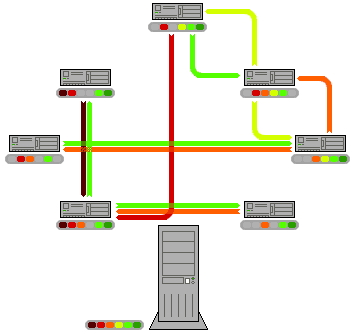
\includegraphics[width=\textwidth]{Torrentcomp_small-4.png}}
        \caption{}
        \label{fig:torrent-repr-4}
    \end{subfigure}%
    \quad
    \begin{subfigure}[H]{\myhsize}
        \fbox{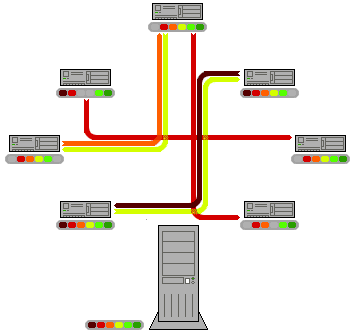
\includegraphics[width=\textwidth]{Torrentcomp_small-5.png}}
        \caption{}
        \label{fig:torrent-repr-5}
    \end{subfigure}

    \vspace{\myvsize}

    \begin{subfigure}[H]{\myhsize}
        \fbox{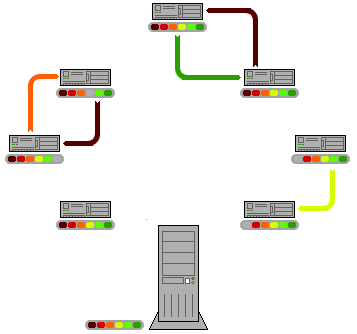
\includegraphics[width=\textwidth]{Torrentcomp_small-6.png}}
        \caption{}
        \label{fig:torrent-repr-6}
    \end{subfigure}%
    \quad
    \begin{subfigure}[H]{\myhsize}
        \fbox{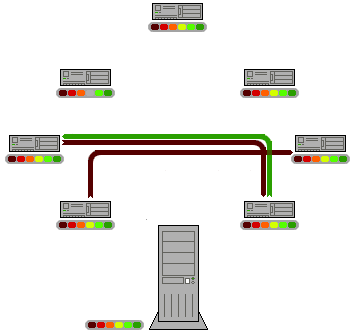
\includegraphics[width=\textwidth]{Torrentcomp_small-7.png}}
        \caption{}
        \label{fig:torrent-repr-7}
    \end{subfigure}%
    \quad
    \begin{subfigure}[H]{\myhsize}
        \fbox{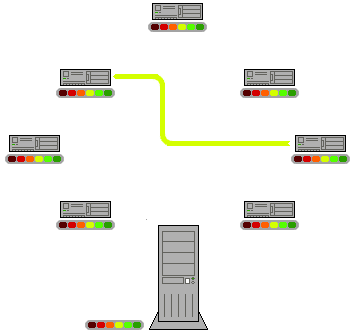
\includegraphics[width=\textwidth]{Torrentcomp_small-8.png}}
        \caption{}
        \label{fig:torrent-repr-8}
    \end{subfigure}

    \vspace{\myvsize}

    \begin{subfigure}[H]{\myhsize}
        \fbox{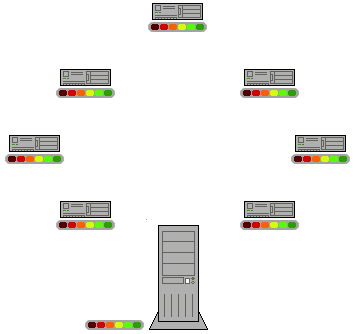
\includegraphics[width=\textwidth]{Torrentcomp_small-9.png}}
        \caption{}
        \label{fig:torrent-repr-9}
    \end{subfigure}

    % TODO: trocar menos (-) por hífen (--)
    \caption{simulação de uma transferência torrent: o seeder, na parte
    inferior das figuras, possui todas as 5 partes de um arquivo, que os outros
    computadores - os leechers - baixam de forma independente e paralela. Fonte:
    \cite{fig:torrent-dl}}
    \label{fig:torrent-repr}
\end{figure}

Todos esses agentes possuem relações múltiplas entre si. Por exemplo, um mesmo
\gls*{torrentfile} pode estar indexado por vários sites indexadores. Como veremos
nos capítulos seguintes, eles contêm uma informação que os identificam unicamente,
gerando consistência entre esses vários sites de busca. Outra observação a ser feita é
que um \gls*{peer} pode estar baixando um ou mais \glspl*{torrent} simultaneamente, ou
seja, participando de vários \glspl*{swarm} ao mesmo tempo. Por fim, em alguns casos,
um mesmo \gls*{torrent} pode possuir uma grande quantidade de \glspl*{peer}
participantes, havendo necessidade de dividí-los em vários \glspl*{swarm}, para fins de
escalabilidade da rede formada.

\begin{figure}[H]
    \centering
    \fbox{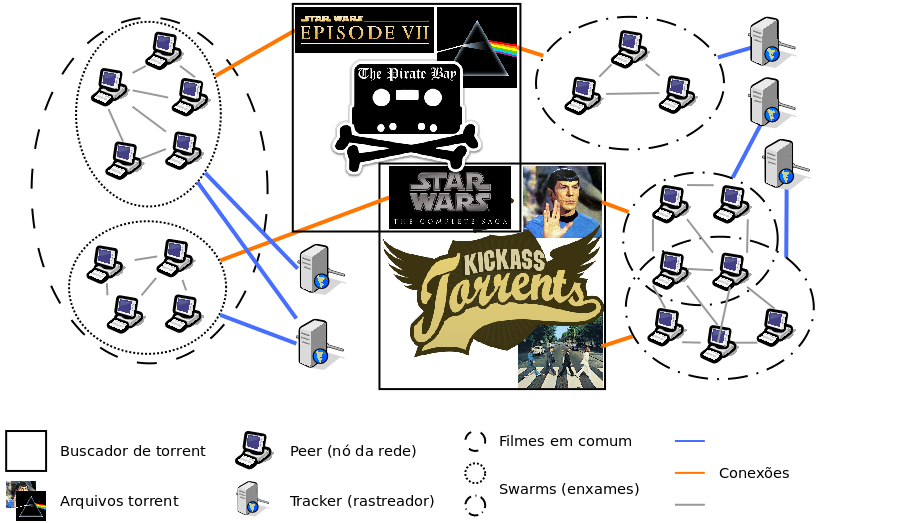
\includegraphics[width=0.85\textwidth]{universobt.png}}
    \caption{amostra de uma rede de conexões BitTorrent}
    \label{fig:torrent-universo}
\end{figure}

\newpage
\subsection*{Arquivo .torrent}

Ao se adicionar um \gls*{torrentfile} em um programa cliente, ocorrem muitas
transmissões de dados antes do download de fato. Para demonstrar isso, usaremos um
\gls*{torrentfile} do filme ``A Noite dos Mortos Vivos'', de 1960 \cite{torrent-file},
que é de domínio público e livre de direitos autorais.

Se abrirmos esse arquivo, veremos uma grande \gls{string}, caracteres diferentes e
incomuns, formando um conteúdo ilegível (na seção binária) e sob uma forma compacta,
mostrado abaixo.

\begin{listing}[H]
    \begin{minted}[
        linenos,
        frame=single,
        numbersep=6pt,
        baselinestretch=1,
        fontfamily=courier,
        gobble=4,
        fontsize=\scriptsize
    ]{text}
    d8:announce36:http://bt1.archive.org:6969/announce13:announce-listll36:http://bt1.
    archive.org:6969/announceel36:http://bt2.archive.org:6969/announceee7:comment13:crea
    tiondatei1343715473e4:infod5:filesld5:crc328:030208fe6:lengthi4127671704e3:md532:627
    f5a428f9e454ccfcb29d31b87169a5:mtime10:10794024804:pathl29:night_of_the_living_dead.
    mpege4:sha140:5e44bb1b3f700240249a5287c64dc02dc56d034bee4:name24:night_of_the_living
    _dead12:piecelengthi4194304e6:pieces23720:<binary>

    (...)

    e6:locale2:en5:title24:night_of_the_living_dead8:url-listl28:http://archive.org/
    download/39:http://ia600301.us.archive.org/22/items39:http://ia700301.us.archive.
    org/22/itemsee
    \end{minted}

    \caption{trecho do conteúdo do arquivo .torrent do filme ``A Noite dos Mortos
    Vivos'', de 1960 \cite{torrent-file}, com a parte binária truncada}
    \label{lst:torrent-file-raw}
\end{listing}

Esse conteúdo está organizado usando a \gls{bencode}, que é uma codificação compacta de
arquivos, especial para \glspl*{torrentfile}, e ininteligível. Com alguma formatação,
podemos enxergar os componentes separadamente, como mostra o código
~\ref{lst:torrent-file-code}.

Esse conteúdo tem significado, sendo utilizado da seguinte forma
\cite{wikitheory:bencoding}:

\begin{itemize}
    \item \textbf{\glspl*{string}} são prefixos de números na base 10, que representam
        comprimentos, seguidos por um caractere \bverb|:| e então o conteúdo. Por
        exemplo, na linha 2, \bverb|8:announce| corresponde à \gls*{string}
        \sverb|"announce"|.

    \item \textbf{números} são representados por um \bverb|i|, seguidos do valor na
        base 10 (sem qualquer limite de tamanho, mas sem zeros precedentes - como em
        \bverb|0003| - e pode ser negativo), terminados por um \bverb|e|. Por exemplo,
        na linha 11, \bverb|i1343715473e| corresponde ao número \sverb|1343715473|.

    \item \textbf{listas} são formadas por \bverb|l|, seguidos por seus elementos
        (também no formato \gls*{bencode}), e então terminados por \bverb|e|. Por
        exemplo, \bverb|l3:foo3:bare| corresponde a \sverb|["foo", "bar"]|. No código
        ~\ref{lst:torrent-file-code}, é presente entre as linhas 43 e 47.

    \item \textbf{dicionários} são definidos por \bverb|d|, seguidos de uma lista
        alternada de chaves e seus valores correspondentes, terminando com \bverb|e|,
        onde as chaves devem estar ordenadas usando-se comparação binária, ao invés da
        usual alfanumérica. Por exemplo, a \gls*{string}
        \bverb|d3:foo3:bar6:foobar6:bazbare| corresponde ao dicionário puro \\
        \sverb|{"foo": "bar", "foobar": "bazbar"}|, e a estrutura mais complexa dada por
        \\ \bverb|d3:fool6:foobar3:bazee| equivale a \sverb|{"foo": ["foobar", "baz"]}|.
\end{itemize}

\begin{listing}[H]
    \begin{minted}[
        linenos,
        frame=single,
        numbersep=6pt,
        baselinestretch=1,
        fontfamily=courier,
        gobble=4,
        fontsize=\scriptsize
    ]{text}
    d
        8:announce
        36:http://bt1.archive.org:6969/announce
        13:announce-list
        l
            l36:http://bt1.archive.org:6969/announcee
            l36:http://bt2.archive.org:6969/announcee
        e
        7:comment
        13:creation date
        i1343715473e
        4:info
        d
            5:files
            l
                d
                    5:crc32
                    8:030208fe
                    6:length
                    i4127671704e
                    3:md5
                    32:627f5a428f9e454ccfcb29d31b87169a
                    5:mtime
                    10:1079402480
                    4:path
                    l29:night_of_the_living_dead.mpege
                    4:sha1
                    40:5e44bb1b3f700240249a5287c64dc02dc56d034b
                e
            e
            4:name
            24:night_of_the_living_dead
            12:piece length
            i4194304e
            6:pieces
            23720:<binary>
        e
        6:locale
        2:en
        5:title
        24:night_of_the_living_dead
        8:url-list
        l
            28:http://archive.org/download/
            39:http://ia600301.us.archive.org/22/items
            39:http://ia700301.us.archive.org/22/items
        e
    e
    \end{minted}
    \caption{trechos formatados de forma legível do conteúdo do arquivo .torrent do
    filme ``A Noite dos Mortos Vivos'', de 1960 \cite{torrent-file}, com a parte
    binária truncada}
    \label{lst:torrent-file-code}
\end{listing}

\subsection*{Magnet Link}

Além do \gls*{torrentfile}, existe uma outra forma de se obter os \glspl*{metadata}
necessários para se iniciar a transmissão, utilizando-se de \glspl{magnetlink}.

\Glspl*{magnetlink}, ao contrário dos \glspl*{torrentfile}, não estão gravados em
algum dispositivo de armazenamento. Basicamente, é um esquema de \gls{uri}, usado
exclusivamente para o protocolo.

No caso citado, o site de origem do \gls*{torrentfile} que estamos usando não fornece um
\gls*{magnetlink} oficialmente. Porém, o Transmission consegue construir uma \gls*{uri}
a partir do arquivo original, para fins de compartilhamento direto. O resultado, após
decodificar o endereço para um formato legível (retirando a \gls{urlencode})
\cite{wiki:urlencode}, foi o seguinte:

\begin{listing}[ht!]
    \begin{minted}[
        linenos,
        frame=single,
        numbersep=6pt,
        baselinestretch=1,
        fontfamily=courier,
        gobble=4,
        fontsize=\scriptsize
    ]{text}
    magnet:?xt=urn:btih:72d7a3179da3de7a76b98f3782c31843e3f818ee
    &dn=night_of_the_living_dead
    &tr=http://bt1.archive.org:6969/announce&tr=http://bt2.archive.org:6969/announce
    &ws=http://archive.org/download/
    &ws=http://ia600301.us.archive.org/22/items/&ws=http://ia700301.us.archive.org/22/items/
    \end{minted}
    \caption{link magnético do arquivo .torrent do filme ``A Noite dos Mortos Vivos''
    , de 1960 \cite{torrent-file}, com parâmetros divididos entre linhas para melhor
    visualização}
    \label{lst:torrent-file-magnet-link}
\end{listing}

Esse endereço é composto por vários pares, compostos por nomes de parâmetros e seus
respectivos valores, sem qualquer ordem específica, formando uma \gls{querystring}.
Podemos dividir esse endereço em partes, cada uma tendo o seu significado:

\begin{itemize}
    \item \textbf{xt}: parâmetro para \emph{exact topic}, ou tópico exato, que contém a
        informação mais importante do \gls*{magnetlink}: o identificador único de
        \glspl*{torrent}. Serve para encontrar e verificar os arquivos especificados.
        No caso, \bverb|urn:btih:<hash>| corresponde ao \gls{urn} \sverb|btih|
        (\emph{BitTorrent Info Hash}), que é a \gls*{string} \gls{hashvalue} resultado
        da \gls{hashfunction} SHA-1, convertida para hexadecimal;

    \item \textbf{dn}: parâmetro que contém o \emph{display name}, ou nome de
        visualização, que é um texto de apresentação amigável para o usuário;

    \item \textbf{tr}: o \emph{address tracker}, ou endereço do \gls*{tracker}, onde o
        programa cliente vai procurar as informações de \glspl*{peer};

    \item \textbf{ws}: endereço do arquivo para \emph{webseed}, ou fornecimento web,
        que é o endereço de Internet de um servidor HTTP ou FTP, que será utilizado como
        alternativa a um \gls*{swarm} problemático \cite{wiki:torrent};
\end{itemize}

\section{Busca por informações}

Quando adicionamos um \gls*{torrent} ao Transmission, o programa salva as
informações em disco durante todo o período em que estas estiverem sendo gerenciadas
por ele. Caso tenha sido por meio de um \gls*{torrentfile}, uma cópia deste é salva em
uma pasta pré-definida para seu controle interno; caso seja por \gls*{magnetlink}, um
novo arquivo é criado contendo as informações obtidas através dele (por questões de
praticidade), para que não necessite fazer essa aquisição dos dados novamente ao ser
aberto, ou quando alguma transferência for pausada e depois continuada.

Após esse arquivamento, o programa processa as informações salvas para deixá-las
carregadas em memória, a fim de obter o \gls*{hashvalue} que identifica o
\gls*{torrentfile}.

\cfile[label="./libtransmission/metainfo.c:367"]{./Codes/chap3/001-leiturametadata.c}

Se aquele arquivo para controle interno tiver sido criado por conta de um
\gls*{magnetlink}, não possuirá a chave \bverb|info| em seu dicionário, mas deverá
conter as chaves \bverb|urn:btih:<hash>| e \bverb|info_hash|.

\cfile[label="./libtransmission/metainfo.c:367"]{./Codes/chap3/002-leiturametadata2.c}

Porém, se o arquivo para controle interno tiver sido criado como cópia do
\gls*{torrentfile}, possuirá o mesmo dicionário, que contém a chave \bverb|info_hash|,
que é utilizada para calcular o \gls*{hashvalue} do arquivo.

\cfile[label="./libtransmission/metainfo.c:367"]{./Codes/chap3/003-leiturametadata3.c}

Outras informações podem ser recuperadas, dependendo da origem do \gls*{torrentfile},
tais como a privacidade do \gls*{torrent}, a lista de arquivos e seus respectivos
tamanhos, \gls*{hashvalue} de cada parte, entre outras. Por fim, termina coletando os
\glspl{announce}.

\cfile[label="./libtransmission/metainfo.c:367"]{./Codes/chap3/004-leiturametadata4.c}

\subsection*{Announce}

Para cada \gls*{swarm} gerenciado, o \gls*{tracker} possui uma lista dos \glspl*{peer}
que participam dele, que é enviada ao \gls*{peer} que a requer por meio de uma
\gls{httpget}. Quando essa requisição é recebida pelo \gls*{tracker}, este incluirá ou
atualizará um registro para o \gls*{peer} solicitante, e devolverá uma lista de 50
\glspl*{peer} aleatórios, de forma uniforme, que fazem parte do \gls*{swarm}. Não
havendo essa quantidade total, a lista toda será enviada ao requisitante. Caso
contrário, a aleatoriedade proporcionará uma diversidade de listas enviadas,
ocasionando robustez ao sistema \cite{wikitheory:tracker-response}.

Esse contato entre um \gls*{peer} e um \gls*{tracker} é chamado de \gls{announce}, que
pode ser feito usando-se tanto o \gls{tcp}, bem como o \gls{udp}, e é como \glspl*{peer}
podem passar várias informações, usando um dicionário no formato \gls*{bencode}:

\begin{itemize}
    \item \textbf{info\_hash}: \gls*{hashvalue} de 20 bytes resultante da
    \gls*{hashfunction} SHA-1, com \gls*{urlencode}, do valor da chave \bverb|info| do
    arquivo \gls*{torrentfile};

    \item \textbf{peer\_id}: \gls*{string} de 20 bytes, com \gls*{urlencode}, usado como
    identificador único do programa cliente, gerado no ínício da sua execução. Para
    isso, provavelmente deverá incorporar informações do computador, a fim de se gerar
    um valor único;

    \item \textbf{uploaded}: a quantidade total de dados, em bytes, enviados desde o
    momento em que o cliente enviou o primeiro aviso ao \gls*{tracker};

    \item \textbf{downloaded}: a quantidade total de dados, em bytes, recebidos desde
    momento em que o cliente enviou o primeiro aviso ao \gls*{tracker};

    \item \textbf{left}: a quantidade total de dados, em bytes, que faltam para o
    requisitante terminar o download do \gls*{torrent} e passe a ser um \gls*{seeder};

    \item \textbf{compact} (opcional): se o valor passado for 1, significa que o
    requisitante aceita respostas compactas. A lista de \glspl*{peer} enviada é
    substituída por uma única \gls*{string} de peers, sendo que cada \gls*{peer} terá
    6 bytes, onde os 4 bytes iniciais são o host e os 2 bytes finais são a porta de
    transmissão. Por exemplo, o endereço IP 10.10.10.5:80 seria transmitido como
    \bverb|0A 0A 0A 05 00 80|. Deve-se observar que alguns \glspl*{tracker} suportam
    somente conexões deste tipo para otimização da utilização da banda de rede e, para
    isso, ou recusarão requisições sem \bverb|compact=1| ou, caso não as recusem,
    enviarão respostas compactas a menos que a requisição possua \bverb|compact=0|;

    \item \textbf{no\_peer\_id} (opcional): sinaliza que o \gls*{tracker} pode omitir o
    campo \textcolor{Bittersweet}{\texttt{peer\_id}} no dicionário de \glspl*{peer},
    porém será ignorado caso o modo compacto esteja habilitado;

    \item \textbf{event} (opcional): pode possuir os valores \sverb|started|
    (iniciado), \sverb|completed| (terminado), \sverb|stopped| (parado), ou vazio para
    não especificar.

    \begin{itemize}
        \item \emph{started} : a primeira requisição para o \gls*{tracker} deve enviar
        este valor;
        \item \emph{stopped} : avisa que o programa cliente está fechando;
        \item \emph{completed} : quando o download que estava ocorrendo termina numa
        mesma execução do programa cliente (não é enviado quando o programa cliente é
        iniciado com o \gls*{torrent} em 100\%);
    \end{itemize}

    \item \textbf{port} (opcional): o número da porta de conexão que o programa cliente
    está escutando por transmissões de dados. Em geral, portas reservadas para
    BitTorrent estão entre 6881 e 6889. Se esse for o caso, pode ser omitido;

    \item \textbf{ip} (opcional): o endereço IP verdadeiro do requisitante, no formato
    legível do IPv4 (4 conjuntos de número de 0 a 255 separados por \bverb|.|) ou do
    IPv6 (8 conjuntos de números hexadecimais de 4 dígitos separados por \bverb|:|).
    Não é sempre necessário, pois o endereço pode ser conhecido através da requisição.
    Assim, é usado quando o programa cliente está se comunicando com o \gls*{tracker}
    através de um \gls{proxy} ou quando ambos (cliente e \gls*{tracker}) estão no mesmo
    lado local de um roteador - com \gls{nat} -, pois, nesse caso o endereço IP não é
    roteável;

    \item \textbf{numwant} (opcional): quantidade de \glspl*{peer} que o requisitante
    gostaria de receber do \gls*{tracker}. É permitido valor zero. Se omitido, assumirá
    valor padrão de 50;

    \item \textbf{key} (opcional): mecanismo de identificação adicional para o programa
    cliente provar sua identidade, caso tenha ocorrido mudança no seu endereço IP;

    \item \textbf{trackerid} (opcional): se a resposta de um \gls*{announce} anterior
    continha o endereço IP de um \gls*{tracker}, deve ser enviado neste campo;
\end{itemize}

%\newpage
\cfile[label="./libtransmission/announcer-common.h:127"]{./Codes/chap3/005-announcestruct.c}
\cfile[label="./libtransmission/announcer.c:1200"]{./Codes/chap3/006-announce.c}

Como resposta, é recebida um outro dicionário em \gls*{bencode}, podendo conter as
seguintes chaves:

\begin{itemize}
    \item \textbf{failure\_reason}: se presente, não podem existir outras chaves no
    dicionário. Seu valor é uma \gls*{string} de mensagem de erro legível sobre o
    porque a requisição falhou;

    \item \textbf{warning\_message} (opcional): similar à chave
    \bverb|failure\_reason|, mas com a requisição tendo sido processada normalmente. A
    mensagem é mostrada como um erro;

    \item \textbf{interval}: intervalo, em segundos, que o cliente deve esperar emtre
    requisições de \gls*{announce} ao \gls*{tracker};

    \item \textbf{min\_interval} (opcional): intervalo mínimo, em segundos, entre
    requisições de \gls*{announce}. Se presente, o pragrama cliente não deve efetuar
    essas requisições acima da frequência estipulada;

    \item \textbf{tracker\_id}: \gls*{string} que o programa cliente deve enviar de
    volta nas próximas requisições. Se ausente e um valor tiver sido passado
    anteriormente, o uso desse valor antigo é continuado;

    \item \textbf{complete}: quantidade de \glspl*{seeder};

    \item \textbf{incomplete}: quantidade de \glspl*{leecher};

    \item \textbf{peers}: pode ser uma das opções

    \begin{enumerate}
        \item lista de dicionários \gls*{bencode}, com as seguintes chaves:

        \begin{itemize}
            \item \textbf{peer\_id}: identificador de um \gls*{peer} na forma de
            \gls*{string}, escolhido por si próprio da mesma forma que a descrito pela
            definição de requisição;

            \item \textbf{ip}: endereço IP do \gls*{peer} nos formatos IPv4 (4 octetos)
            ou IPv6 (valores hexadecimais), ou ainda o nome de domínio DNS (string);

            \item \textbf{port}: número da porta utilizada pelo \gls*{peer};
        \end{itemize}

        \item \gls*{string} binária cujo tamanho é de 6 bytes para cada \gls*{peer},
        onde os 4 primeiros representam o endereço IP e os 2 últimos são o número da
        porta, em notação de rede (\emph{big endian});
    \end{enumerate}
\end{itemize}

\begin{listing}[H]
    \begin{minted}[
        linenos,
        frame=single,
        numbersep=6pt,
        baselinestretch=1,
        fontfamily=courier,
        gobble=4,
        fontsize=\scriptsize
    ]{text}
    * About to connect() to exodus.desync.com port 6969 (#8)
    *   Trying 208.83.20.164...
    *
    * Connected to exodus.desync.com (208.83.20.164) port 6969 (#8)
    > GET /announce?info_hash=\%88\%15\%8c\%7bW\%e0\%85\%21\%86~\%d0\%b5\%de\%06\%5b\%
    7dWI\%cf\%d7&peer_id=-TR2820-ne1joqgh8z9o&port=51413&uploaded=0&downloaded=0&left=52
    406288292&numwant=80&key=6ee99240&compact=1&supportcrypto=1&requirecrypto=1&event=
    started HTTP/1.1
    User-Agent: Transmission/2.82
    Host: exodus.desync.com:6969
    Accept: */*
    Accept-Encoding: gzip;q=1.0, deflate, identity

    < HTTP/1.1 200 OK
    < Content-Type: text/plain
    < Content-Length: 136
    <
    * Connection #8 to host exodus.desync.com left intact
    Announce response:
    < {
        "complete": 1,
        "downloaded": 11,
        "incomplete": 6,
        "interval": 1732,
        "min interval": 866,
        "peers": \"<binary>\"
    }
    \end{minted}

    \caption{Logs do Transmission sobre uma requisição de announce e a respectiva
    resposta, com o conteúdo binário truncado}
    \label{lst:announce}
\end{listing}

Essa comunicação ocorre nas seguintes situações:

\begin{itemize}
    \item no primeiro contato do \gls*{peer}, para que ele tenha acesso a um
        \gls*{swarm};

    \item a cada período de tempo, estipulado pelo tracker, para que o \gls*{peer}
        continue mostrando que ainda está conectado, além de poder receber endereços de
        \glspl*{peer} novos;

    \item quando a quantidade de \glspl*{peer} conhecidos que estiverem ativos for
        menor do que 5;

    \item quando terminar o download, notificando que passou a ser um \gls*{seeder};

    \item quando sair do \gls*{swarm}, seja por desconexão ou por encerramento do
        programa cliente;
\end{itemize}

\subsection*{Scrape}

Além do \gls*{announce}, outra forma de troca de informação entre \glspl*{peer} e
\glspl*{tracker} se dá pelo \gls{scrape}. Geralmente usado pelos programas cliente para
decidir quando realizar um \gls*{announce}, informa o número de \glspl*{peer},
\glspl*{leecher} e \glspl*{seeder} de uma lista de um ou mais \glspl*{torrent}. É dessa
forma que os sites de indexação sabem dessas informações e as apresentam nas em páginas.

A requisição de \gls*{scrape} pode ser sobre todos os \glspl*{torrent} que o
\gls*{tracker} gerencia ou sobre um ou mais \glspl*{torrent} em específico, quando são
passados seus respectivos \glspl*{hashvalue}. Sua resposta é um dicionário na forma
\gls*{bencode} contendo as chaves

\begin{itemize}
    \item \textbf{files}: um dicionário contendo um par chave-valor para cada
    \gls*{torrent} especificado na requisição do \gls*{scrape} através do
    \gls*{hashvalue} do \gls*{torrent} de 20 bytes:

    \begin{itemize}
        \item \textbf{complete}: quantidade de \glspl*{seeder};

        \item \textbf{incomplete}: quantidade de \glspl*{leecher};

        \item \textbf{downloaded}: quantidade total de vezes que o \gls*{tracker}
        registrou uma finalização (\sverb|event=complete| ao término de um download);

        \item \textbf{name} (opcional): o nome interno do \gls*{torrent}, como
        especificado pelo respectivo \gls*{torrentfile}, na sua seção \bverb|info|;
    \end{itemize}
\end{itemize}

Da mesma forma que o \gls*{announce}, o \gls*{scrape} é um endereço do \gls*{tracker}
usando-se o \gls*{tcp} ou o \gls*{udp}, e é tratado de forma semelhante pelo Transmission.

\cfile[label="./libtransmission/announcer-common.h:37"]{./Codes/chap3/007-scrapestruct.c}
\cfile[label="./libtransmission/announcer.c:1397"]{./Codes/chap3/008-scrape.c}

\begin{listing}[H]
    \begin{minted}[
        linenos,
        frame=single,
        numbersep=6pt,
        baselinestretch=1,
        fontfamily=courier,
        gobble=4,
        fontsize=\scriptsize
    ]{text}
    * About to connect() to www.mvgroup.org port 2710 (#1)
    *   Trying 88.129.153.50...
    * Connected to www.mvgroup.org (88.129.153.50) port 2710 (#1)
    > GET /scrape?info_hash=\%83F\%24\%b62\%e5Q\%cc4\%10h\%ba\%1e8\%e2C\%f7\%80\%01\%87 HTTP/1.1
    User-Agent: Transmission/2.82
    Host: www.mvgroup.org:2710
    Accept: */*
    Accept-Encoding: gzip;q=1.0, deflate, identity

    * HTTP 1.0, assume close after body
    < HTTP/1.0 200 OK
    <
    * Closing connection 1
    Scrape response:
    < {
        "files": {
            \"<binary>\": {
                "complete": 9,
                "downloaded": 59074,
                "incomplete": 2
            }
        }
    }
    \end{minted}

    \caption{Logs do Transmission sobre uma requisição de scrape e a respectiva
    resposta, com o conteúdo binário truncado}
    \label{lst:scrape}
\end{listing}

\subsection*{Convenção de scrape de trackers}

O endereço de \gls*{scrape} pode ser obtido a partir do endereço de \gls*{announce},
seguindo-se a seguinte convenção:

\begin{enumerate}
    \item comece a partir do endereço de \gls*{announce}

    \item encontre o último caractere \bverb|/|

    \item se o texto que segue a última \bverb|/| não for \sverb|announce|, é um sinal
    que o \gls*{tracker} não segue a convenção

    \item caso contrário, substituir \sverb|announce| por \sverb|scrape|
\end{enumerate}

Alguns exemplos:

\begin{itemize}
    \item suportam \sverb|scrape|
        \begin{enumerate}
            \item \url{http://example.com/announce} $\rightarrow$ \url{http://example.com/scrape}
            \item \url{http://example.com/announce.php} $\rightarrow$ \url{http://example.com/scrape.php}
            \item \url{http://example.com/x/announce} $\rightarrow$ \url{http://example.com/x/scrape}
            \item \url{http://example.com/announce?x2\%0644} $\rightarrow$ \url{http://example.com/scrape?x2\%0644}
        \end{enumerate}

    \item não suportam \sverb|scrape|
        \begin{enumerate}
            \item \url{http://example.com/a}
            \item \url{http://example.com/announce?x=2/4}
            \item \url{http://example.com/x\%064announce}
        \end{enumerate}
\end{enumerate}

%\section{Fontes de arquivos}

Com a requisição do \gls*{announce}, o Transmission recebe a sua resposta e prepara
esses dados para utilização, carregando-os em memória.

\cfile[label="./libtransmission/announcer-http.c:288"]{./Codes/chap3/009-httpannounce.c}
\cfile[label="./libtransmission/announcer-http.c:189"]{./Codes/chap3/010-onhttpannouncedone.c}

Após essa preparação dos dados da resposta do \gls*{announce}, cuja informação
principal é a lista de \glspl*{peer}, o Transmission gerencia o tempo para a próxima
requisição periódica de \gls*{announce} ou \gls*{scrape}. Além disso, sinaliza para a
\gls{thread} principal do programa que recebeu a resposta do \gls*{tracker}.

\cfile[label="./libtransmission/announcer.c:1012"]{./Codes/chap3/011-onannouncedone.c}
\cfile[label="./libtransmission/announcer.c:523"]{./Codes/chap3/012-publicapeers.c}

A \gls*{thread} principal percebe que foi sinalizado o recebimento de uma resposta de
\gls*{tracker} e começa a utilizar a lista de \glspl*{peer} adquirida, adicionando-os ao
\gls{pool} do objeto em memória que representa o \gls{swarm}.

\cfile[label="./libtransmission/torrent.c:552"]{./Codes/chap3/013-ontrackerresponse.c}
\cfile[label="./libtransmission/peer-mgr.c:2113"]{./Codes/chap3/014-addpex.c}

Essa inclusão é condicionada ao fato de que o endereço de um \gls*{peer} ainda não está
contido na lista de \glspl*{peer}.

\cfile[label="./libtransmission/peer-mgr.c:1852"]{./Codes/chap3/015-verificapeer.c}

Assim, a lista de \glspl*{peer} do Transmission está pronta para ser utilizada nos
pedidos das partes do \gls*{torrent}.

\newpage
\section{Tabelas Hash Distribuídas e o Kademlia}

Os \glspl{dht} surgiram quando buscas em \glspl{p2p} não eram eficientes, fosse pelos
problemas da supercentralização dos sistemas ou pela falta dela, tentando criar uma
maneira híbrida de buscar e localizar recursos nessas redes.

Existem duas formas de se encontrar objetos: busca e endereçamento. A primeira se baseia
no casamento de palavras-chave com as das descrições dos objetos, sendo mais amigável
para um usuário pois não necessita de formas complexas de identificação. Porém, é mais
difícil de se tornar eficiente, além de precisar conferir também os objetos para saber
se são o mesmo. As \glspl*{p2p} descentralizadas utilizavam desta abordagem.

A segunda, no entanto, utiliza endereços que possam identificá-los de forma única. Dessa
forma, um objeto é exclusivamente identificável, sendo possível encontrá-lo
eficientemente. Contudo, é necessário algum procedimento de se conhecer seu nome único,
além de ser requerido manter uma estrutura organizada por endereços. Historicamente, as
\glspl*{p2p} de estrutura centralizada se baseavam neste método.

Uma outra maneira de organizar esses objetos através da rede é de organizar as conexões
entre os diversos \glspl*{peer}, que acabam formando redes superpostas (\emph{overlay
networks}), que são redes virtuais que figuram sobre as tradicionais redes IP.

Anteriormente ao BitTorrent, nas \glspl*{p2p} de estrutura centralizada, o servidor
central tentava conhecer a situação de cada um dos \glspl*{peer} da rede, enviando
mensagens diretamente a eles. Gerenciar muitos \glspl*{peer} ao mesmo tempo
sobrecarregava o \emph{hardware} do servidor, ou forçava o seu desligamento. Por outro
lado, quando a rede tinha estrutura descentralizada, ocorria o fenômeno chamado de
inundação de mensagens, no qual estas eram repassadas entre \glspl*{peer}
intermediários até o \gls*{peer} de destino. Esse repasse excessivo acarretava
sobrecarga de processamento (\emph{overhead}) dos intermediários, além de gerar
mensagens falso-negativas.

Assim, as \glspl*{p2p} necessitam de funcionalidades eficientes para que um \gls*{peer}
possa entrar e sair do \emph{overlay}, assim como armazenar objetos e encontrá-los
(usando endereçamento). Tal eficiência é conseguida através de \glspl{dht}, onde todas
essas funcionalidades dependem da troca de mensagens eficiente entre \glspl*{peer}.

\begin{figure}[H]
    \centering
    \fbox{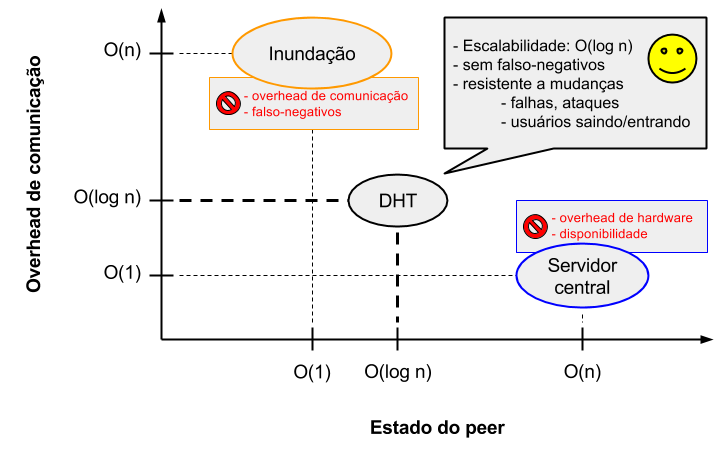
\includegraphics[width=0.85\textwidth]{graph-dht.png}}
    %\caption{amostra de uma rede de conexões BitTorrent}
    %\label{fig:torrent-universo}
\end{figure}

\subsection*{Kademlia}

O Kademlia é um \gls*{dht} criado em 2002 \cite{artigo:kademlia} com o objetivo de
melhorar os métodos de busca atuais (Napster e\gls*{gnutella}), que eram ineficientes.
Assim como os outros algoritmos de \gls*{dht}, ele se baseou na estrutura informalmente
conhecida como ``rede de Plaxton'' (\emph{Plaxton mesh}), nome que remete a um dos seus
autores \cite{artigo:dht}. Por ter causado boas impressões, foi usado na implementação
da busca de arquivos no programa cliente eMule.

O algoritmo implementa uma rede \emph{overlay} cuja estrutura e comunicação se baseiam
na procura de seus nós. Cada um destes nós é identificado por um identificador único
(ID), que serve tanto para a identificação quanto para a localização de valores na
\gls*{hashtable}. Durante uma busca, o processo deve conhecer a chave (que é um
\gls*{hashvalue}) associado ao objeto - neste caso, o ID do \gls*{torrent}, que é seu
\gls*{hashvalue} - e explora a rede em passos, encontrando nós mais próximos da chave,
até encontrar o valor buscado ou não nós existirem mais próximos que o atual. Dessa
forma, para uma rede com $n$ nós, o algoritmo visita apenas $O(\log n)$ nós.

\subsection*{Funcionamento}

No Kademlia, objetos e nós possuem IDs únicos de 160 bits: enquanto o primeiro utiliza
o \gls*{hashvalue} de 20 bytes SHA-1 da chave \bverb|info_hash| do \gls*{torrentfile},
o segundo é um valor aleatório escolhido pelo próprio programa.

Como este \gls*{dht} é construído com base em distâncias entre nós, a função de medida
escolhida foi

\begin{equation}
    d(x,y) = x \oplus y
\end{equation}

pois possui algumas propriedades em comum com a equação de distância euclidiana usual.
Assim, seguem suas propriedades:

\begin{itemize}
    \item $d(x,x) = 0$
    \item $x \neq y$, $d(x,y) > 0$
    \item simetria: $\forall x,y$, $d(x,y) = d(y,x)$
    \item desigualdade triangular: $d(x,y) + d(y,z) \geq d(x,z)$. \\
        Isto vem do fato de $d(x,z) = d(x,y) \oplus d(y,z)$ e que $\forall a \geq 0,
        \forall b \geq 0 : a + b \geq a \oplus b$
    \item unidirecionalidade: para um dado ponto $x$ e uma distância $\Delta > 0$,
        existe exatamente um ponto $y$ tal que $d(x,y) = \Delta$. Isso garante que todas
        as procuras por uma mesma chave convirjam para um mesmo percurso, independente
        do ponto de partida.
\end{itemize}

\subsubsection*{Estado dos nós}

Cada nó do Kademlia armazena informações sobre outros nós para rotear mensagens de
pesquisa. Para cada bit dos IDs (cada ID tem 160 bits) é mantido um $k$-bucket, que é
uma lista de triplas ordenada pelo horário da última notícia do \gls*{peer} listado,
contendo seu endereço IP, porta de comunicação \gls*{udp} e o ID, para os nós cuja
distância para ele está entre $2^i$ e $2^{i+1}$. Para distâncias pequenas, essas listas
geralmente serão vazias, enquanto para distâncias maiores poderão ser de tamanho $k$.
Este valor, que é o de replicação do sistema, é escolhido de tal forma que, para dados
quaisquer $k$ nós sejam improváveis de falharem na próxima hora.

\subsubsection*{Protocolo}

%\todo[inline]{explicar teoria}

\section{Peer Exchange}

\todo[inline]{Funciona somente no \gls*{swarm}!}
tuplas
\todo[inline]{Explicar a funcionalidade de PEX}

\section{Jogo da troca de arquivos}
\label{titfortat}

Explicarei o algoritmo tit-for-tat padrão do protocolo BitTorrent, que vem da Teoria dos Jogos, e como o Transmission o implementa.

\afterpage{\clearpage} % Anatomia

%!TEX root = ../tcc.tex

\chapter{Conceitos de Computação no BitTorrent}

\todo[inline]{Fazer pequena introdução aqui.}
Aqui mostrarei detalhes técnicos sobre as partes coadjuvantes do BitTorrent e do Transmission.


\section{Estruturas de dados, listas ligadas e árvores}
\section{Funções de hash} % SHA1
\section{Criptografia} %RC4
\section{Bitfields}
\section{Protocolos de redes} % HTTP e UDP
\section{Multicast}
\section{Roteamento de pacotes} %NAT PMP
\section{IPv6}
\section{Retomada de downloads}
\section{Conexão com a Internet}
\section{Threads}
\section{Engenharia de Software}

\afterpage{\clearpage}
 % Parte técnica

%!TEX root = ../tcc.tex

\chapter{Transmission e o BCC}

Neste texto descrevemos que são encontradas vários elementos de Ciência da Computação no
programa cliente Transmission. A intensão agora é encontrar quais disciplinas da grade
curricular do Bacharelado em Ciência da Computação (BCC) da perpectiva dos conhecimentos
utilizados no Transmission.

\begin{figure}[H]
    \centering
    \fbox{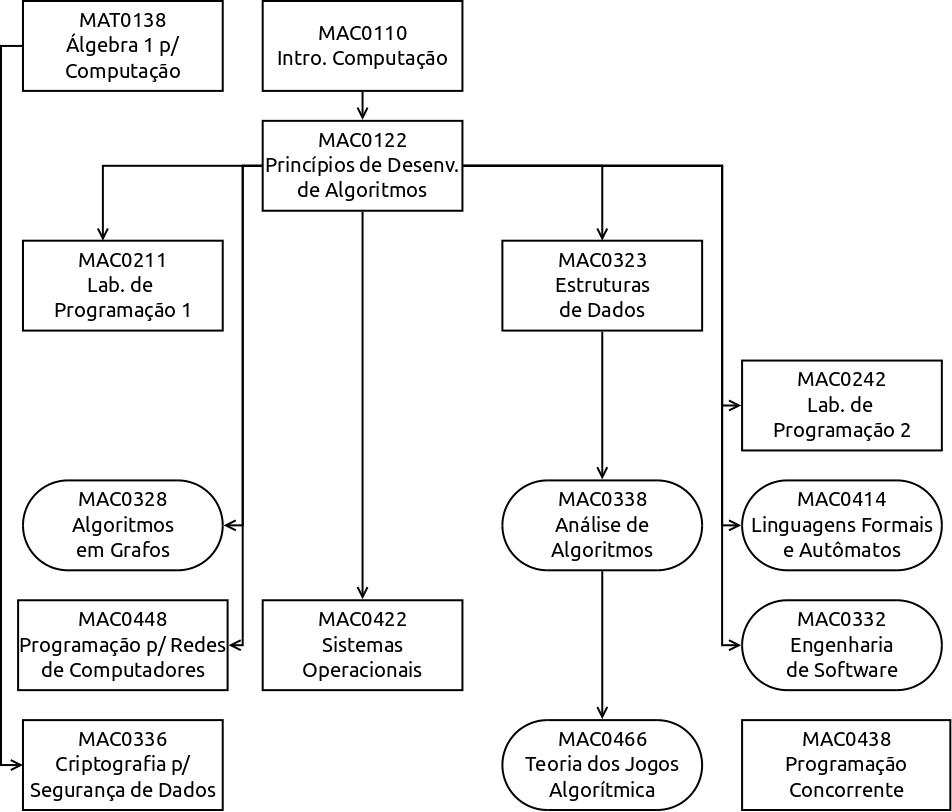
\includegraphics[width=.75\textwidth]{mapa-bcc.png}}
    \caption{disciplinas do BCC utilizadas diretamente na programação do Transmission, ligadas pelos seus pré-requisitos. As bordas arredondadas indicam que o conhecimento auxilia, mas não é necessário.}
    \label{fig:bcc}
\end{figure}

Das disciplinas do BCC, as reconhecidas como necessárias para o entendimento do
BitTorrent e o Transmission foram:

\begin{itemize}
    \item Intro. à Computação (MAC0110), Princípios de Desenvolvimento de Algoritmos
        (MAC0122), Laboratórios de Programação 1 (MAC0211): linguagem C, organização de
        código, trabalho gerenciado em grupos de desenvolvedores, portabilidade de
        código entre plataformas (Autoconf e Automake);

    \item Estruturas de Dados (MAC0323): utilização e manipulação de estruturas de
        dados, como vetores e listas ligadas;

    \item Algoritmos em Grafos (MAC0328): entendimento do algoritmo de busca de nós no
        \gls{dht};

    \item Análise de Algoritmos (MAC0328) e Teoria dos Jogos Algorítmica (MAC0446):
        algoritmo da troca das partes entre \glspl{peer};

    \item Álgebra 1 (MAT0138) e Criptografia para Segurança de Dados (MAC0336): noções
        de álgebra modular e seus usos nos métodos criptográficos;

    \item Laboratório de Programação 2 (MAC0242) e Engenharia de Software (MAC0332):
        desenvolvimento de programas complexos;

    \item Programação para Redes (MAC0448): desenvolvimento de código de conexão via
        Internet, como \gls{tcp} e \gls{udp}, multicast, \gls{nat}, IPv6, UPnP e
        \gls*{nat}-pmp;

    \item Linguagens Formais e Autômatos (MAC0414): uso de autômatos para entendimento
        dos estados dos \glspl*{peer} e suas transições com as trocas de mensagens
        \cite{conf:swarming}; e

    \item Sistemas Operacionais (MAC0422) e Programação Concorrente (MAC0438): uso de
        \glspl{thread} e métodos para computação com seus usos, como acesso à memória
        compartilhada (\emph{mutex}) e travas, e entendimento de caches de memória na
        leitura e escrita de dados.
\end{itemize}

\afterpage{\clearpage} % Conclusão

%!TEX root = ../tcc.tex

\nocite{*}
\printbibliography % Referências

%!TEX root = ../tcc.tex

\chapter{Visão Pessoal}


\clearpage
 % Parte Subjetiva

% Espaço no ToC, por estética
% \addtocontents{toc}{\vspace{2em}}

\end{document}
